\documentclass[../CSC_52081_EP.tex]{subfiles}

\begin{document}
\section{Results and Discussion}

\subsection{DQN and SARSA Comparison}

The evolution curve of the models can be seen in Figures \ref{fig:DQN_evolution} and \ref{fig:SARSA_evolution}, respectively. The blue curve shows the episodic rewards, while the orange line represents the moving average, providing a clearer view of the overall learning trend.

The DQN was trained over 2300 episodes. The reward curve shows an upward trend, indicating that the DQN is learning and improving its policy over time. The reward stabilizes around 820 ± 171.98 by episode 2364, suggesting that the model has likely converged to a near-optimal policy, and the steady improvement suggests that the learning rate is likely well-tuned. Given that the maximum reward reached in the environment is 926.8, the results are quite satisfactory, but the convergence takes more time to saddle.

\begin{figure}[H]
    \centering
    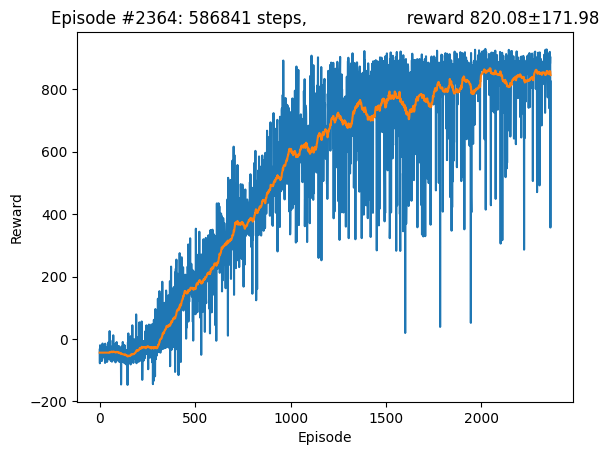
\includegraphics[width=0.3\textwidth]{figures/DQN_train_2364.png}
    \caption{Evolution curve showing the rewards over episodes - DQN for 2300 episodes.}
    \label{fig:DQN_evolution}
\end{figure}


\begin{figure}[H]
    \centering
    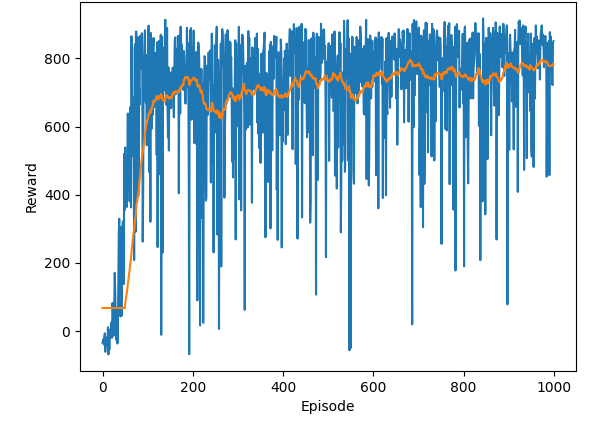
\includegraphics[width=0.3\textwidth]{figures/SARSA_train.png}
    \caption{Evolution curve showing the rewards over episodes - Deep SARSA for 1000 episodes.}
    \label{fig:SARSA_evolution}
\end{figure}

For the SARSA model, 1000 episodes were simulated. The agent starts with low rewards in the early episodes, as expected, while it explores the environment. Rapid improvement occurs within the first 100-200 episodes, showing that the agent is learning a useful policy. After this phase, rewards continue to increase but with fluctuations, which suggest that the learning rate may be moderately high, allowing for quick learning, but eventually stabilizing around 784 ± 126.7.

Overall, this proved to be a good training and the final performance is strong, indicating that the policy has reached a near-optimal state, while also fast and sample-efficient, followed by stable convergence.

In order to compare algorithm performance under the same conditions of an environment (which is randomly generated), we fixed a seed variable upon its generation to maintain the main caracteristics.
We performed five simulations for over 25 seeds. The graph for comparison can be seen in Figure \ref{fig:SARSA_DQN_comparison}.

% \begin{figure}[H]
%     \centering
%     \includegraphics[width=0.3\textwidth]{figures/aaaaaaaa.png}
%     \caption{Average Reward over environment with seeds ranging from 0 to 24, comparison between DQN and Deep SARSA performances.}
%     \label{fig:SARSA_DQN_comparison}
% \end{figure}

In summary, Deep SARSA prioritizes fast adaptation but requires more time to stabilize, while DQN takes longer to learn but ultimately achieves higher performance and stability.

\subsection{CEM}

Figure \ref{fig:train_plot} shows the evolution of the training rewards over iterations for the CEM algorithm. As expected from the minimization strategy applied in our implementation, the reward value starts at a high level and decreases steadily, eventually stabilizing between 5 and 10. This behavior indicates that the algorithm is correctly minimizing the cost, since our objective function returns the negative reward.

\begin{figure}[H]
    \centering
    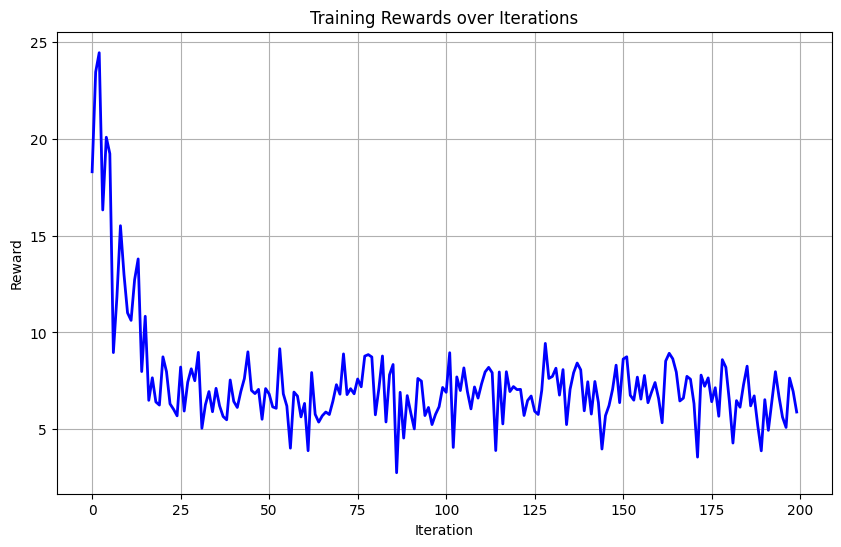
\includegraphics[width=0.3\textwidth]{figures/CEM_train.png}
    \caption{Training plot showing the evolution of the reward over iterations.}
    \label{fig:train_plot}
\end{figure}

However, the desired outcome was to achieve a much lower (more negative) reward value as training progressed, which would have translated into better performance by the agent when navigating the track. Unfortunately, the final model did not produce the expected results in the environment, as demonstrated by the video reproduction of the car on the track.

This may be the result of some problems with the model. One possibility is that the reward structure, when negated for minimization, may be inadvertently favoring a strategy that minimizes penalization rather than encouraging forward progress. Additionally, the parameters of the CNN or the action scaling (especially for the steering, gas, and brake outputs) might not be appropriately tuned, causing the policy to output nearly constant or ineffective actions. Overall, these factors combined may result in the agent exploiting a trivial strategy that minimizes the cost, rather than discovering a policy that drives effectively along the track. But, despite this problem, the training plot confirms that the minimization mechanism is operating as designed.

\subsection{PPO and SAC}

For both algorithms, over approximatly 1000 episodes, we did not observe a tranding that converged to an optimal policy. Figure \ref{fig:PPO_train} shows the poor performance of the model, that can be explained by higher complexity of the continuous action-space possibilities.

\begin{figure}[H]
    \centering
    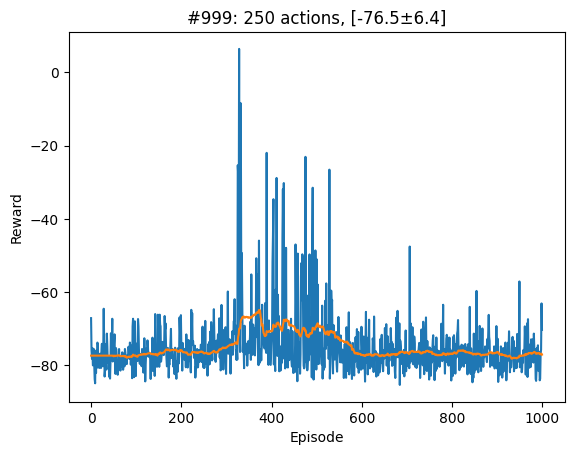
\includegraphics[width=0.3\textwidth]{figures/reward_per_episode_PPO.png}
    \caption{Evolution curve of the rewards per episode for the PPO algorithm.}
    \label{fig:PPO_train}
\end{figure}

We then evaluated both performances of PPO and SAC under the same conditions (same environment), which can be seen in Figure \ref{fig:PPO_SAC_comparison}.

% \begin{figure}[H]
%     \centering
%     \includegraphics[width=0.3\textwidth]{figures/aaaaaaaa.png}
%     \caption{Average Reward over environment, comparison between PPO and SAC algorithms.}
%     \label{fig:PPO_SAC_comparison}
% \end{figure}

Many of the reasons that could explain the poor performance of the algorithms are that continuous action spaces introduce infinitely many possible actions, making exploration harder compared to discrete spaces. If the policy does not explore effectively, it may fail to find optimal actions.
PPO and SAC are highly sensitive to hyperparameters like learning rate, entropy regularization (SAC), and clipping ratio (PPO). Inappropriate values can lead to either premature convergence to suboptimal policies or unstable training.
Additionally, the neural networks may struggle to approximate the optimal policy in complex continuous spaces, especially if architecture, activation functions, or regularization are not well chose, and there are many possibilities.

Overall, we don't have enough evidence to claim that the algorithm completly failed, because analysing the videos after 1000 episodes, it does seem to make reasonable choices, but is not fast enough. Maybe with more training it would start to perform better, but we did not have the time to train the algorithm (usually it requires more than 10 hours).


\end{document}
